\chapter*{}

\Huge{\centering \textsc{Burning geometric graphs}\\~\\~\\~\\~\\}

\begin{figure}[h]
	\begin{minipage}{1\textwidth}
		\centering
		\subfigure[]{
		    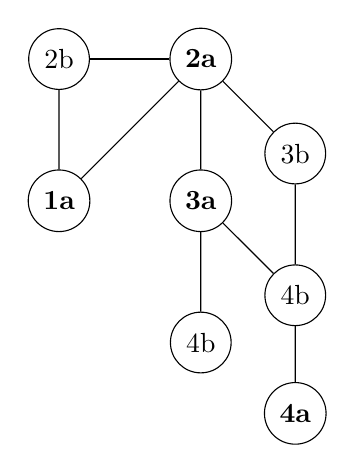
\begin{tikzpicture}[scale=.6]
			    \node[draw,shape=circle] (AA) at (-8,0) {2b};
		    	\node[draw,shape=circle] (AB) at (-5,0) {\textbf{2a}};
		    	\node[draw,shape=circle] (AC) at (-8,-3) {\textbf{1a}};
		    	\node[draw,shape=circle] (AD) at (-5,-3) {\textbf{3a}};
		    	\node[draw,shape=circle] (AE) at (-3,-2) {3b};
		    	\node[draw,shape=circle] (AF) at (-5,-6) {4b};
		    	\node[draw,shape=circle] (AG) at (-3,-5) {4b};
		    	\node[draw,shape=circle] (AH) at (-3,-7.5) {\textbf{4a}};
		    	
		    	\draw (AA)--(AB);
		    	\draw (AA)--(AC);
		    	\draw (AB)--(AC);
		    	\draw (AB)--(AD);
		    	\draw (AB)--(AE);
		    	\draw (AE)--(AG);
		    	\draw (AD)--(AF);
	    	    \draw (AD)--(AG);
	    	    \draw (AG)--(AH);
		    \end{tikzpicture}
		}
		\subfigure[]{
		    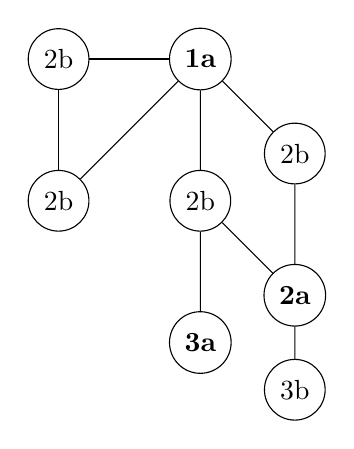
\begin{tikzpicture}[scale=.6]
		    	\node[draw,shape=circle] (BA) at (8-8,0) {2b};
		    	\node[draw,shape=circle] (BB) at (8-5,0) {\textbf{1a}};
		    	\node[draw,shape=circle] (BC) at (8-8,-3) {2b};
		    	\node[draw,shape=circle] (BD) at (8-5,-3) {2b};
		    	\node[draw,shape=circle] (BE) at (8-3,-2) {2b};
		    	\node[draw,shape=circle] (BF) at (8-5,-6) {\textbf{3a}};
		    	\node[draw,shape=circle] (BG) at (8-3,-5) {\textbf{2a}};
		    	\node[draw,shape=circle] (BH) at (8-3,-7) {3b};
		    	
		    	\draw (BA)--(BB);
		    	\draw (BA)--(BC);
		    	\draw (BB)--(BC);
		    	\draw (BB)--(BD);
		    	\draw (BB)--(BE);
		    	\draw (BE)--(BG);
		    	\draw (BD)--(BF);
	    	    \draw (BD)--(BG);
	    	    \draw (BG)--(BH);
		    \end{tikzpicture}
		}
    \end{minipage}\\~\\~\\~\\~\\~\\~\\
\end{figure}

\begin{flushright}
\large{\textsc{Arya Tanmay Gupta}}
\end{flushright}